\documentclass[11pt,a4paper]{article}
\oddsidemargin 0.1 cm \evensidemargin 0.1cm \textwidth 16cm
\textheight24cm
\setlength{\topmargin}{0pt}\setlength{\headsep}{0pt}\pagestyle{empty}

\usepackage{graphicx}
\usepackage{variations}
\usepackage{enumerate}
\usepackage{amssymb}
\usepackage[latin1]{inputenc}  
\usepackage{fontenc}   
\usepackage{amsmath}
\usepackage{amsthm}
\usepackage{amsthm}
\usepackage{xypic}
\usepackage{variations}
%\usepackage{fancyhdr}
%\usepackage{xcolor}
%\usepackage{pstricks-add}
\usepackage[francais]{babel}
%\usepackage[french]{babel}
\newtheorem{defi}{D\'{e}finition}
\newtheorem{thm}{Th\'{e}or\`{e}me}
\newtheorem{rmq}{Remarque}
\newtheorem{prop}{Propri\'{e}t\'{e}}
\newtheorem{prop-def}{Propri\'{e}t\'{e}-D\'{e}finition}
\newtheorem{ex}{Exemple}
\newtheorem{exs}{Exemples}
\newtheorem{exer}{Exercice}
%\newtheorem{proof}{D\'{e}monstration}
\def\di{\displaystyle}
\newcommand{\vtab}{\rule[-0.4em]{0pt}{1.2em}}
\usepackage[top=0.5cm,bottom=0.5cm,right=1.5cm,left=1.5cm]{geometry}
\usepackage{pstricks,pst-plot} 
%\usepackage{framed}
\usepackage{amsmath}
%\usepackage{amssymb}
\usepackage{fancyhdr}
\usepackage{fancybox}
\usepackage{multicol}
%\usepackage{xcolor}
\usepackage{epsfig}
\usepackage{pifont}
%\usepackage[framed]{ntheorem}
%\usepackage[frenchb]{babel}
\usepackage{tabularx}
\def\R{{\mathbb R}}
\newtheorem{Rem}{Remarque}
\newcommand{\V}{\overrightarrow}
\newcommand{\Rep}{(O;\V{\imath};\V{\jmath})}
\newcommand{\Coor}[2]{\begin{pmatrix} #1\\#2 \end{pmatrix}}

\begin{document}
\title{}         % Enter your title between curly braces
\author{}        % Enter your name between curly braces
\date{}          % Enter your date or \today between curly braces
\maketitle

\indent\vspace{-3.5cm}
$$\fbox{\text{\begin{Large}Colin�arit� de vecteurs - Feuille d'exercices\end{Large}}}$$
     
\hfill\\[0.2cm]

\noindent\underline{\textbf{Exercice 1 :}}\\ 
$ABC$ est un triangle �quilat�ral de c�t� $3$ cm.
Placer les points $D$ et $E$ tels que $\V{AD}=-2\V{AB}$ et $\V{AE}=\di\frac{1}{2}\V{BC}$.
\hfill\\


\noindent\underline{\textbf{Exercice 2 :}} On consid�re la figure ci-contre.\\
\begin{minipage}{0.6\linewidth}
\begin{enumerate}
\item D�terminer les r�els $k$ et $k'$ tels que :
$$\V{AM}=k\V{AB} \ \ \ \text{et} \ \ \ \V{AN}=k' \V{AC}$$
\item Compl�ter par le nombre r�el qui convient :\\[0.2cm]
\begin{minipage}{0.5\linewidth}
\begin{enumerate}[$\diamond$]
\item $\V{MA}= ......... \V{MB}$
\item $\V{NC}= ......... \V{NA}$
\end{enumerate}
\end{minipage}
\begin{minipage}{0.4\linewidth}
\begin{enumerate}[$\diamond$]
\item $\V{BM}= ......... \V{MA}$
\item $\V{AC}= ......... \V{NA}$
\end{enumerate}
\end{minipage}
\end{enumerate}
\end{minipage}
\begin{minipage}{0.4\linewidth}
\hfill\\[-1cm]
$$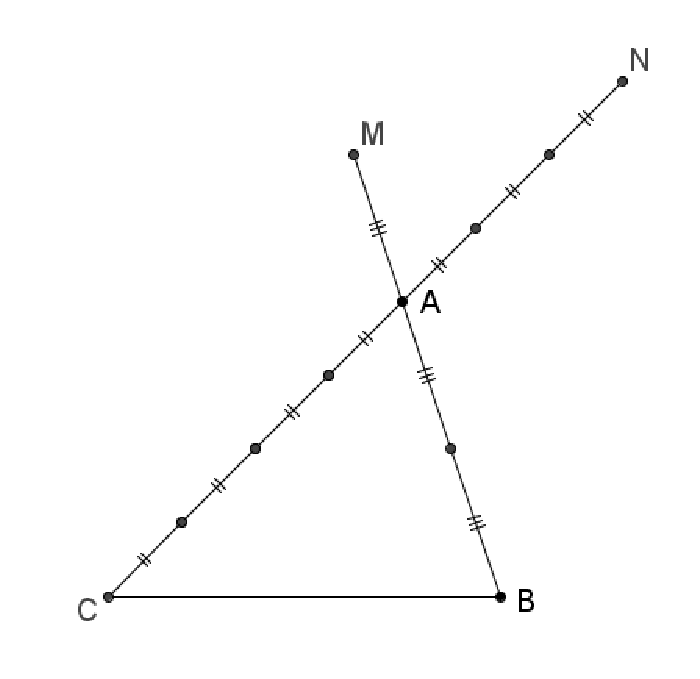
\includegraphics[scale=0.5]{exo2.eps}$$
\end{minipage}
\hfill\\[-0.4cm]

\noindent\underline{\textbf{Exercice 3 :}}\\
Soient $A$ et $B$ deux points distincts du plan et soit $I$ le milieu de $[AB]$. Dans chacun des cas suivants, compl�ter par le nombre r�el $k$ qui convient :
$$ \V{AI}=.......... \ \V{AB} \ \  ; \ \ \V{AI}=.......... \ \V{IB} \ \ ; \ \ \V{BI}=.......... \ \V{AB}$$
\hfill\\[-0.4cm]


\noindent\underline{\textbf{Exercice 4 :}}\\
Soit $ABC$ un triangle. Placer les points $E$, $F$, $G$ et $H$ tels que :
$$\V{AE}=\V{AB}+2\V{AC} \ \ ; \ \ \V{AF}=-2\V{AB}+\V{AC} \ \ ; \ \ \V{AG}=2\V{AB}+3\V{AC} \ \ ; \ \ \V{AH}=-3\V{AB}+\V{BC}$$
\hfill\\[-0.4cm]



\noindent\underline{\textbf{Exercice 5 :}}\\
Soit $ABCD$ un parall�logramme. Soient $I$ et $J$ les milieux respectifs des c�t�s $[AB]$ et $[CD]$.
\begin{enumerate}
\item D�montrer que $\V{AJ}=\V{IC}$. Que peut-on en d�duire pour $(AJ)$ et $(IC)$ ?
\item D�montrer que les droites $(DI)$ et $(JB)$ sont parall�les.
\end{enumerate}
\hfill\\[-0.4cm]

\noindent\underline{\textbf{Exercice 6 :}}\\ 
Soit $ABC$ un triangle. Soient $I$, $J$ et $K$ les milieux respectifs des c�t�s $[AB]$, $[AC]$ et $[BC]$.\\
D�terminer le r�el $k$ tel que $\V{BC}=k\V{IJ}$.
\hfill\\


\noindent\underline{\textbf{Exercice 7 :}}\\
Soit $[AB]$ un segment de longueur $8$ cm. On cherche � construire un point $M$ tel que $\V{MA}+3\V{MB}=\V{0}$
\begin{enumerate}
	\item D�montrer, en utilisant la relation de Chasles, que l'�galit� ci-dessus s'�crit aussi :
	$$4\V{MA}+3\V{AB}=\V{0}$$
	\item En d�duire l'expression de $\V{AM}$ en fonction de $\V{AB}$ et construire le point $M$.
\end{enumerate}
\hfill\\



\noindent\underline{\textbf{Exercice 8 :}}\\
Soit $ABC$ un triangle. Soient $I$ le milieu de $[BC]$ et $G$ le centre de gravit� du triangle $ABC$. Compl�ter par le nombre r�el qui convient :
\begin{enumerate}[$\diamond$]
	\item $\V{AG}= .......... \ \V{AI}$ ;\\[-0.2cm]
	\item $\V{GI}= .......... \ \V{AI}$ ;\\[-0.2cm]
	\item $\V{GA}= .......... \ \V{GI}$.
\end{enumerate}
\hfill\\













\end{document}
